\documentclass{sigkddExp}
\usepackage{etoolbox}
\makeatletter
\patchcmd{\@sect}{\vskip -14pt}{}{}{\errmessage{main_kdd.tex: could not patch the heading spacing in \string\@sect}}
\def\@copyrightspace{}%
\makeatother

\usepackage[utf8]{inputenc}
\usepackage[T1]{fontenc}
\usepackage{cite}
\usepackage{amsmath,amssymb}
\usepackage{graphicx}
\usepackage{booktabs}
\usepackage{multirow}
\usepackage{tabularx}
\usepackage{array}
\usepackage[table]{xcolor}
\usepackage{pifont}
\usepackage[nointegrals]{wasysym}
\usepackage{tikz}
\usetikzlibrary{shapes,positioning,fit,backgrounds,arrows.meta,decorations.pathreplacing}
\usepackage{fontawesome5}
\usepackage{url}
\usepackage{xurl}
\providecommand{\thepage}{\arabic{page}}

\usepackage[hidelinks]{hyperref}
\hypersetup{pdftitle={A Survey on Jev: Prior Research, Adaptation Costs, and Evidence of System One Models},pdfauthor={Evan Chen, Jiamu Zhang, Tianze Yang, Kelly Wan, Liangjie Hong, Liang Wu}}

\setlength{\emergencystretch}{1.5em}
\makeatletter
\def\section{\@startsection{section}{1}{\z@}{-10\p@ \@plus -4\p@ \@minus -2\p@}%
  {4\p@}{\baselineskip 14pt\secfnt\@ucheadtrue\raggedright}}
\def\subsection{\@startsection{subsection}{2}{\z@}{-8\p@ \@plus -2\p@ \@minus -\p@}%
  {4\p@}{\secfnt\raggedright}}
\makeatother

\newcommand{\axisM}{\textsf{M}}
\newcommand{\axisD}{\textsf{D}}
\newcommand{\axisC}{\textsf{C}}
\newcommand{\rev}[1]{#1}

\definecolor{axisMc}{HTML}{2A78D6}   %
\definecolor{axisDc}{HTML}{EB6834}   %
\definecolor{axisCc}{HTML}{1BAF7A}   %
\definecolor{seriesTypedc}{HTML}{4A3AA7} %
\definecolor{seriesLLMc}{HTML}{E87BA4}   %
\definecolor{goodc}{HTML}{0CA30C}
\definecolor{critc}{HTML}{D03B3B}
\definecolor{inkc}{HTML}{0B0B0B}
\definecolor{mutedc}{HTML}{52514E}
\colorlet{tblheadc}{mutedc!14}       %
\colorlet{tblgroupc}{mutedc!7}       %

\setlength{\aboverulesep}{0pt}
\setlength{\belowrulesep}{0pt}
\setlength{\extrarowheight}{1.6pt}

\renewcommand{\axisM}{\textcolor{axisMc}{\textsf{\textbf{M}}}}
\renewcommand{\axisD}{\textcolor{axisDc}{\textsf{\textbf{D}}}}
\renewcommand{\axisC}{\textcolor{axisCc}{\textsf{\textbf{C}}}}

\newcommand{\cyes}{\textcolor{inkc}{\textnormal{\CIRCLE}}}
\newcommand{\cpart}{\textcolor{inkc}{\textnormal{\LEFTcircle}}}
\newcommand{\cno}{\textcolor{mutedc}{\textnormal{\Circle}}}
\newcommand{\cna}{\textcolor{mutedc}{--}}

\newcommand{\vok}{\textcolor{goodc}{\ding{51}}}        %
\newcommand{\vbad}{\textcolor{critc}{\ding{55}}}       %
\newcommand{\vopen}{\textcolor{mutedc}{\textbf{?}}}     %

\newcommand{\tblhead}{\rowcolor{tblheadc}}
\newcommand{\tblgroup}[2]{\rowcolor{tblgroupc}\multicolumn{#1}{@{}l}{\hspace{2pt}\textsc{#2}}\\}
\newcommand{\thd}[1]{\textbf{#1}}

\pdfstringdefDisableCommands{%
  \def\axisM{M}\def\axisD{D}\def\axisC{C}}

\providecommand{\glyphLab}{\ensuremath{\bullet}}          %
\providecommand{\glyphProf}{\ensuremath{\blacklozenge}}   %
\providecommand{\glyphWarm}{\ensuremath{\blacktriangle}}  %
\providecommand{\glyphSpec}{\ensuremath{\star}}           %
\providecommand{\glyphAll}{\ensuremath{\boxplus}}         %

\newcommand{\dmp}{\texttt{decision-\allowbreak{}model-\allowbreak{}preview}}


\begin{document}

\title{A Survey on Jev: Prior Research, Adaptation Costs, and Evidence of System One Models}

\numberofauthors{1}
\author{
\alignauthor Evan~Chen, Jiamu~Zhang, Tianze~Yang, Kelly~Wan, Liangjie~Hong and Liang~Wu\\
       \affaddr{Nokia, Sunnyvale, CA, USA}%
\thanks{Nokia develops AnyJev. \rev{All authors are authors of the AnyJev technical report, and E.~Chen is also an author of CARGO.} Both systems are discussed in this survey.}\\
       \affaddr{\{evan.chen, jiamu.zhang, tianze.yang, kelly.wan, liangjie.hong, liang.wu\}@nokia.com}
}

\maketitle

\begin{abstract}

Many decisions in LLM systems do not need generated text. They only need a choice among a few fixed options, such as which model should handle a request or whether a response is safe. Typed decision models, also called Jev-style or System One decision models, are designed for exactly this case. They take a state and a question specified at call time, and instead of generating text, they return a probability distribution over a closed answer set. TypeSafe AI offers this interface in Jev, and several open implementations reproduce it. This short survey explains what these models are, where their ideas come from, and what the current evidence can support. These models build on earlier work, which we organize into two areas of earlier research. The first area, routing research, supplies the goal: a decision component that adapts when the system changes, without retraining. The second area supplies the mechanisms: zero-shot classifiers, safety guards, and label-probability readout. How much ``no retraining'' actually saves, however, depends on what changes. We therefore examine the adaptation cost of three kinds of change: new models, new decisions, and new deployment constraints. Adding a new candidate model is not free, because the routing approaches reviewed here still rely on candidate-specific evidence for each new candidate. A new type of decision, however, can be specified without retraining the shared model. Finally, a new deployment constraint, such as a target error rate, still requires labeled examples. The empirical evidence is also mixed. On the positive side, independent studies report valid outputs and large cost reductions compared with LLM judges, although these savings shrink when the baseline is already cheap. On the negative side, the same studies find that accuracy trails frontier LLMs on hard tasks, that calibration varies across workloads and subgroups, and that added context can change decisions. Given these trade-offs, we recommend testing a typed model against two simpler alternatives before adopting it: a label-probability readout on an open model, and a cheap generative cascade. The comparison should use the same acceptance rule the deployment will use.
 

\end{abstract}

\keywords{\interlinepenalty=10000 Jev, typed decision models, System One models, LLM routing, zero-shot classification, calibration, selective prediction, guardrails.\par}

\section{Introduction}
\label{sec:intro}
\begin{figure}[t]
\centering
\resizebox{\columnwidth}{!}{%
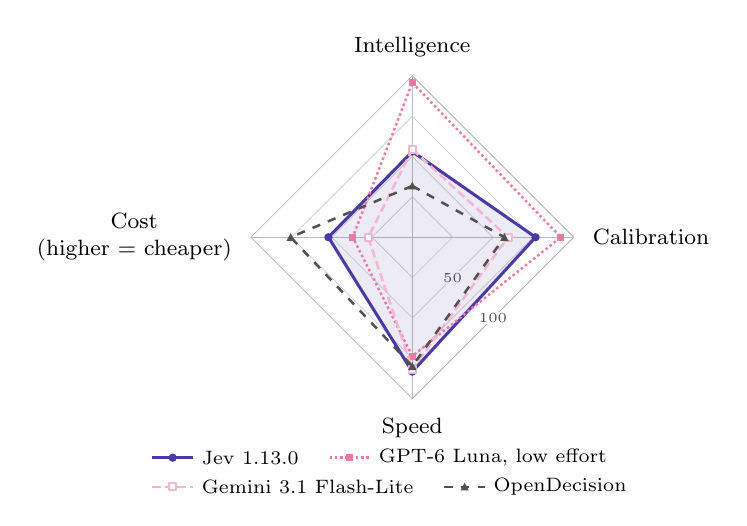
\begin{tikzpicture}[font=\scriptsize, line join=round]
  \def\R{2.05}
  \colorlet{seriesTyped}{seriesTypedc}
  \colorlet{seriesLLM}{seriesLLMc}
  \draw[mutedc!25, line width=0.3pt] (0,0.25*\R) -- (0.25*\R,0) -- (0,-0.25*\R) -- (-0.25*\R,0) -- cycle;
  \draw[mutedc!25, line width=0.3pt] (0,0.50*\R) -- (0.50*\R,0) -- (0,-0.50*\R) -- (-0.50*\R,0) -- cycle;
  \draw[mutedc!25, line width=0.3pt] (0,0.75*\R) -- (0.75*\R,0) -- (0,-0.75*\R) -- (-0.75*\R,0) -- cycle;
  \draw[mutedc!45, line width=0.3pt] (0,1.00*\R) -- (1.00*\R,0) -- (0,-1.00*\R) -- (-1.00*\R,0) -- cycle;
  \node[font=\tiny, text=mutedc, fill=white, inner sep=0.6pt] at (-45:0.50*\R*0.7071) {50};
  \node[font=\tiny, text=mutedc, fill=white, inner sep=0.6pt] at (-45:1.00*\R*0.7071) {100};
  \foreach \a in {90,0,-90,180}{ \draw[mutedc!40, line width=0.3pt] (0,0) -- (\a:\R); }
  \node[anchor=south, align=center, font=\footnotesize] at (90:{\R+0.12}) {Intelligence};
  \node[anchor=west, align=center, font=\footnotesize] at (0:{\R+0.12}) {Calibration};
  \node[anchor=north, align=center, font=\footnotesize] at (-90:{\R+0.12}) {Speed};
  \node[anchor=east, align=center, font=\footnotesize] at (-180:{\R+0.12}) {Cost\\(higher = cheaper)};
  \draw[seriesTyped, line width=1.1pt, fill=seriesTyped, fill opacity=0.10] (90:0.5306*\R) -- (0:0.7634*\R) -- (-90:0.8327*\R) -- (-180:0.5197*\R) -- cycle;
  \fill[seriesTyped] (90:0.5306*\R) circle (1.5pt);
  \fill[seriesTyped] (0:0.7634*\R) circle (1.5pt);
  \fill[seriesTyped] (-90:0.8327*\R) circle (1.5pt);
  \fill[seriesTyped] (-180:0.5197*\R) circle (1.5pt);
  \draw[seriesLLM, line width=0.9pt, densely dotted] (90:0.9578*\R) -- (0:0.9198*\R) -- (-90:0.7366*\R) -- (-180:0.3689*\R) -- cycle;
  \fill[seriesLLM] ([shift={(-1.3pt,-1.3pt)}]90:0.9578*\R) rectangle ++(2.6pt,2.6pt);
  \fill[seriesLLM] ([shift={(-1.3pt,-1.3pt)}]0:0.9198*\R) rectangle ++(2.6pt,2.6pt);
  \fill[seriesLLM] ([shift={(-1.3pt,-1.3pt)}]-90:0.7366*\R) rectangle ++(2.6pt,2.6pt);
  \fill[seriesLLM] ([shift={(-1.3pt,-1.3pt)}]-180:0.3689*\R) rectangle ++(2.6pt,2.6pt);
  \draw[seriesLLM!55, line width=0.9pt, dash pattern=on 3pt off 1.5pt] (90:0.5447*\R) -- (0:0.5929*\R) -- (-90:0.8179*\R) -- (-180:0.2736*\R) -- cycle;
  \draw[seriesLLM!55, fill=white, line width=0.7pt] ([shift={(-1.3pt,-1.3pt)}]90:0.5447*\R) rectangle ++(2.6pt,2.6pt);
  \draw[seriesLLM!55, fill=white, line width=0.7pt] ([shift={(-1.3pt,-1.3pt)}]0:0.5929*\R) rectangle ++(2.6pt,2.6pt);
  \draw[seriesLLM!55, fill=white, line width=0.7pt] ([shift={(-1.3pt,-1.3pt)}]-90:0.8179*\R) rectangle ++(2.6pt,2.6pt);
  \draw[seriesLLM!55, fill=white, line width=0.7pt] ([shift={(-1.3pt,-1.3pt)}]-180:0.2736*\R) rectangle ++(2.6pt,2.6pt);
  \draw[mutedc, line width=0.9pt, dashed] (90:0.3180*\R) -- (0:0.5706*\R) -- (-90:0.7990*\R) -- (-180:0.7534*\R) -- cycle;
  \fill[mutedc] ([shift={(-1.5pt,-1.3pt)}]90:0.3180*\R) -- ++(3pt,0) -- ++(-1.5pt,2.8pt) -- cycle;
  \fill[mutedc] ([shift={(-1.5pt,-1.3pt)}]0:0.5706*\R) -- ++(3pt,0) -- ++(-1.5pt,2.8pt) -- cycle;
  \fill[mutedc] ([shift={(-1.5pt,-1.3pt)}]-90:0.7990*\R) -- ++(3pt,0) -- ++(-1.5pt,2.8pt) -- cycle;
  \fill[mutedc] ([shift={(-1.5pt,-1.3pt)}]-180:0.7534*\R) -- ++(3pt,0) -- ++(-1.5pt,2.8pt) -- cycle;
  \tikzset{legsample/.style={inner sep=0pt, minimum width=0.5cm, minimum height=2.8pt}}
  \node[legsample, anchor=west] (L0) at (-3.3,{-\R-0.75}) {};
  \draw[seriesTyped, line width=1.1pt] (L0.west) -- (L0.east); \fill[seriesTyped] (L0.center) circle (1.5pt);
  \node[right=2pt of L0, inner sep=1pt] (T0) {Jev 1.13.0};
  \node[legsample, right=10pt of T0] (L1) {};
  \draw[seriesLLM, line width=0.9pt, densely dotted] (L1.west) -- (L1.east); \fill[seriesLLM] ([shift={(-1.3pt,-1.3pt)}]L1.center) rectangle ++(2.6pt,2.6pt);
  \node[right=2pt of L1, inner sep=1pt] (T1) {GPT-6 Luna, low effort};
  \node[legsample, anchor=west] (L2) at (-3.3,{-\R-1.12}) {};
  \draw[seriesLLM!55, line width=0.9pt, dash pattern=on 3pt off 1.5pt] (L2.west) -- (L2.east); \draw[seriesLLM!55, fill=white, line width=0.7pt] ([shift={(-1.3pt,-1.3pt)}]L2.center) rectangle ++(2.6pt,2.6pt);
  \node[right=2pt of L2, inner sep=1pt] (T2) {Gemini 3.1 Flash-Lite};
  \node[legsample, right=10pt of T2] (L3) {};
  \draw[mutedc, line width=0.9pt, dashed] (L3.west) -- (L3.east); \fill[mutedc] ([shift={(-1.5pt,-1.3pt)}]L3.center) -- ++(3pt,0) -- ++(-1.5pt,2.8pt) -- cycle;
  \node[right=2pt of L3, inner sep=1pt] (T3) {OpenDecision};
\end{tikzpicture}%
}
\caption{Scores of four systems on JevBench v1.4.2.2~\cite{jevbench2026v1422}, from three classes: a typed decision model (Jev 1.13.0), two prompted LLMs (GPT-6 Luna at low reasoning effort and Gemini 3.1 Flash-Lite) and a zero-shot ModernBERT classifier (OpenDecision). Each axis is the benchmark's 0--100 score on the same decisions. Intelligence is chance-corrected accuracy across the benchmark's tiers, calibration measures how well stated probabilities match outcomes, speed maps latency to a score (100 at 0.1\,s, 80 at 1\,s), and cost maps the price per 1{,}000 decisions to a score, so that higher means cheaper. OpenDecision's speed and cost are the benchmark's estimates rather than measurements. The results file reports no uncertainty estimates. On this snapshot, no system is best on every axis. Against Gemini 3.1 Flash-Lite, the typed decision model scores 1.4 points lower on intelligence and higher on the other three axes. The speed scale is logarithmic: Jev's median latency is 0.65\,s, against 1.44\,s for GPT-6 Luna at low effort. We chose one system per class to compare the classes, not to rank systems. Three open-weight typed models rank above Jev on the benchmark's composite score.}
\label{fig:radar}
\end{figure}


As LLM systems take on tasks that involve several steps, they need to decide how to proceed as well as generate responses. An agent may need to choose which tool to call next and when to stop~\cite{yang2026toward}. The surrounding system may also choose which model should handle a request~\cite{varangotreille2025doing} or whether a proposed action is risky~\cite{liu2026evaluating}. Many of these decisions involve a known set of answers. For the software taking the next step, a choice among those answers can be more useful than an explanation, especially if it comes with a probability that helps determine whether to act or seek further review.

One way to obtain such decisions is to ask the generative LLM already handling the user's request to make them as well. For example, the system could ask that model whether to handle a request itself or pass it to another model. However, using a generative LLM for these decisions has three drawbacks: 1) the caller pays for generating answer tokens and, with reasoning models, for thinking tokens~\cite{sui2025stop}; 2) the returned text must be parsed before software can use it; and 3) any reported confidence needs to be checked for the model, task and output format. Token probabilities can be well calibrated in some formats~\cite{kadavath2022language}.

When the same decision is made repeatedly, a conventional classifier offers another option. It is fast and often accurate, but it is trained for a fixed task and label set. Changing the task or labels often requires adapting the classifier or its output head. For systems whose questions change, the work needed to adapt the decision method therefore matters alongside the cost of each call.

Typed decision models address this need by allowing the caller to specify the question, its answer type and its possible answers at call time. The caller supplies the context to be evaluated, called the \emph{state}, and the model returns a probability for each answer rather than generating text. TypeSafe AI offers this interface in Jev, which it describes as a System One model, after Kahneman's fast, intuitive System~1~\cite{kahneman2011thinking,typesafe2026docs}. We use \emph{typed decision model} for this class, also called Jev-style or System One decision models. Several open implementations expose the same interface~\cite{convai2026laya,palmer2026kev,bespoke2026nimble,mapika2026decider,lee2026semif,nokia2026anyjev}, and OpenAI has announced a related Decisions API in limited preview~\cite{openai2026decisions}.

With these options available, a developer needs to understand both how they differ from existing methods and when they are useful. Fig.~\ref{fig:radar} illustrates the practical comparison: on the reported benchmark snapshot, none of the four systems is best on every axis~\cite{jevbench2026v1422}. This motivates a closer look at the earlier research behind typed decision models, the work required to adapt them to a deployment, and the results reported so far.

Earlier research provides a starting point for this comparison. Typed decision interfaces bring together established methods for classification, reading answer probabilities directly from a model, checking those probabilities against observed outcomes, and deferring uncertain decisions. Tang and Zheng review 28 arXiv papers posted between September 19 and 24, 2026, and relate the interface to these methods, constrained generation, reranking and cascades that pass decisions between models~\cite{tang2026typed}. Two concurrent working drafts also review the area: one follows the development from classical classifiers to Jev, including routing and cascades~\cite{awesomejev2026decisions}, and the other examines calibration, deciding when to accept or defer an answer, and open implementations~\cite{luo2026jev}. Surveys of routing~\cite{varangotreille2025doing,moslem2026dynamic} and LLM judges~\cite{gu2024survey} provide further background on these related tasks. Building on this work, our survey makes three contributions:
\begin{enumerate}
\item \textbf{Connections to earlier research.} We explain these connections from two perspectives: 1) routing motivates adapting a system's decisions to change without retraining the decision model, and 2) classification and answer-probability methods help explain how typed decisions are produced (Section~\ref{sec:lineages}).
\item \textbf{Adaptation cost.} We examine the work needed when a system adds a new model, asks a new kind of question or changes a deployment requirement. We distinguish resources that must be acquired from those that can be reused (Section~\ref{sec:adaptation}).
\item \textbf{Evidence and practical guidance.} We bring together independent evaluations to explain where these models are useful and what deployment risks remain. We then give practitioners a procedure for comparing alternatives on their own tasks (Sections~\ref{sec:evidence}--\ref{sec:guidance}).
\end{enumerate}

\noindent\textbf{Scope and sources.} To connect the recent Jev literature with this earlier work, we searched arXiv, GitHub and official documentation for public sources through September 30, 2026\rev{, and cite a few later studies where they bear directly on a finding}. We combined a name for Jev or its interface (Jev, System One model, typed decision model, decision model) with a term for one surveyed family (LLM routing, cascades, zero-shot classification, policy-conditioned guards, rubric judges, label-token readout, calibration), then followed citations from the works found.

Because most work specific to typed decision models appeared in the preceding two weeks as preprints or repositories, the evidence is still developing. At this moment, Jev has no technical report yet, so our description follows TypeSafe's documentation~\cite{typesafe2026docs}. We distinguish documented interface properties from empirical findings and identify results supported by a single study. We call a study \emph{independent} when its authors neither developed nor funded the system it measures, and attribute results to the researchers who measured them.

\section{Typed Decision Models}
\label{sec:models}

\subsection{The Interface}
\label{sec:jev}

To see how these decisions are expressed in practice, we use Jev~1.13 as a concrete example, following TypeSafe's public documentation~\cite{typesafe2026docs}.

\noindent\textbf{Calls and question types.} A call carries a \emph{state}, which is text, a JSON object or an array of text values. It also carries a set of keyed questions of three types: 1) a \texttt{choice} question selects one option from a caller-defined set of at most 255 options, and the answer gives a probability for every option; 2) a \texttt{score} question places the state on an ordered rubric of 2 to 10 levels, and the answer gives a probability for every level and the probability-weighted level; and 3) a Boolean question, which TypeSafe calls \texttt{noul}, asks whether a statement is true, and the answer is the probability of yes. Types can be mixed in one call. The questions of a call are evaluated against the state independently of one another.

\noindent\textbf{Pricing and versions.} The service is priced per input token, and output tokens are free. The same weights serve every account, so a caller adapts Jev only through the state and the text of its questions. Model aliases resolve to versioned identifiers, and the documentation advises pinning a version whenever thresholds have been tuned. Because the service is hosted, every state is sent to TypeSafe. When the state must stay on the team's own infrastructure, only the open-weight rows of Table~\ref{tab:implementations} apply.

\noindent\textbf{Training.} TypeSafe has published no technical report, weights, parameter count, architecture or description of its training data. Its documentation states that customer requests are not used for training. The one named training method is reinforcement learning for calibrated decisions (RLCD). TypeSafe describes RLCD as training the model to return decisions and calibrated probabilities instead of generated text.

\noindent\textbf{Documented limitations.} Jev reads instructions literally and is unreliable on counting, arithmetic, date comparisons and questions that need several hops of reasoning. Its accuracy falls when the state contains unrelated material. It does not treat the state as hostile, so text in the state can steer its answer. A Boolean question and its negation need not receive complementary probabilities. TypeSafe lists these limitations for \texttt{jev-1.13} and pairs each with a workaround, such as keeping arithmetic in code.

\noindent\textbf{A worked call.} Fig.~\ref{fig:interface} shows one call with illustrative values. The state is an agent's proposed tool call together with the user's request. The caller asks one question of each type, and the model returns one distribution per question. The caller's code then applies a threshold to each answer and combines the results. The thresholds, and the decision to act, abstain or escalate, belong to the caller rather than to the model.

\begin{figure*}[t]
\centering
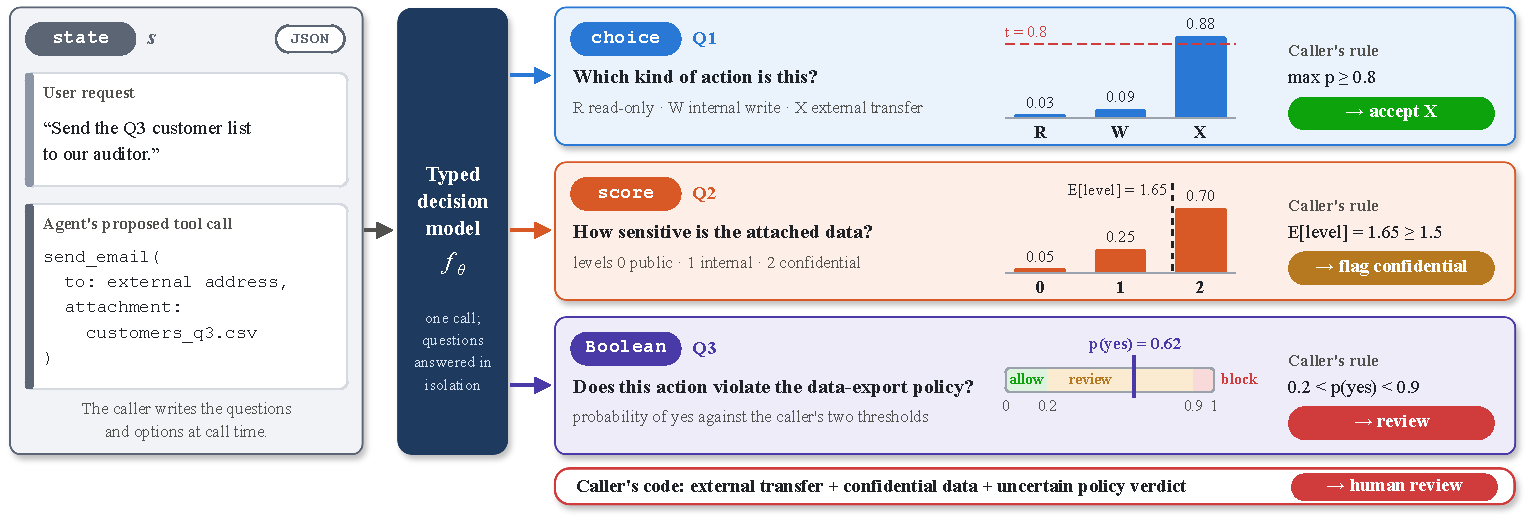
\includegraphics[width=\textwidth]{figures/fig_interface.pdf}
\caption{A worked call to a typed decision model, with illustrative rather than measured values. One state is evaluated against three questions, one of each type. The model returns a distribution over each question's closed answer set: bars show the \texttt{choice} and \texttt{score} distributions, and the Boolean answer is the probability of yes, shown against the caller's allow and block thresholds (shaded band: review). The caller, not the model, sets the thresholds and the rule that combines them.}
\label{fig:interface}
\end{figure*}

\subsection{Properties for Evaluating Typed Decisions}
\label{sec:contract}

We judge a typed decision model by four properties: type safety (P1), calibration (P2), invariance (P3) and cost (P4).

\noindent\textbf{Type safety (P1).} Every answer lies in the declared answer set. This is structural validity, not correctness.

\noindent\textbf{Calibration (P2).} For a \texttt{choice} question, predictions assigned a given top probability should be correct at that rate. The same condition applies to the probability of yes for Boolean questions and to each cumulative event for \texttt{score} questions. Calibration is measured on a deployment distribution, so a model calibrated for one question and one traffic mix need not be calibrated for another, or within every subgroup. The studies in Section~\ref{sec:evidence} report the expected calibration error (ECE), a binned estimate of this gap.

\noindent\textbf{Invariance (P3).} Reordering the options should not change the probability each option receives. Renaming the options while their definitions are held fixed should not change it either. P3 also covers coherence: a question and its negation should receive complementary probabilities.

\noindent\textbf{Cost (P4).} Cost covers forward passes, network round trips, latency and price per decision. Reports should state what the latency includes, for example model time only or the full round trip.

Type safety is an interface requirement. Calibration, invariance and cost describe behavior that must be measured rather than assumed. Constrained decoding also guarantees type safety~\cite{willard2023efficient}, but the model still generates tokens and exposes probabilities only where the provider returns token log-probabilities. LLM judges accept a rubric at call time~\cite{kim2024prometheus2,liu2023geval}, but they usually report a score or verdict, often with a rationale, rather than a calibrated probability~\cite{gu2024survey}.

Software acts on a decision through an \emph{acceptance rule} that the caller sets. A \texttt{choice} is typically executed when its top probability exceeds a threshold and escalated otherwise. A Boolean gate that asks whether an action is unsafe can use two thresholds. It allows the action below the lower one, blocks it above the upper one, and asks for human review in between. When low-confidence decisions are deferred in this way, the model acts as a selective predictor~\cite{geifman2017selective}. We call the share of decisions resolved without human review or escalation the \emph{automation coverage}. For a Boolean gate, it includes both automatic allows and automatic blocks.

\subsection{Implementations}
\label{sec:implementations}
\begin{table}[!t]
\centering
\caption{Implementations of the typed decision interface, grouped by mechanism family. ``User labels'' counts the labeled examples a user supplies per new question to obtain probabilities; developer training data are excluded. Every row still needs labeled evidence to set an acceptance rule for a risk target (Section~\ref{sec:adaptation}). ``Passes'' counts model passes for one question. L0, L1 and L2 are AnyJev's zero-label, temperature-fitted and closed-form-head levels, with label counts as stated by its developers. $K$: number of options.}
\label{tab:implementations}
\footnotesize
\setlength{\tabcolsep}{3pt}
\renewcommand{\arraystretch}{1.05}
\begin{tabularx}{\columnwidth}{@{}>{\raggedright\arraybackslash\hspace{0pt}}p{1.42cm}>{\raggedright\arraybackslash\hspace{0pt}}X>{\raggedright\arraybackslash\hspace{0pt}}p{1.3cm}>{\raggedright\arraybackslash\hspace{0pt}}p{1.75cm}@{}}
\toprule
\tblhead \thd{System} & \thd{Mechanism and training} & \thd{User labels} & \thd{Passes} \\
\midrule
\tblgroup{4}{Hosted, closed weights}
Jev 1.13~\cite{typesafe2026docs} & Vendor-trained with RLCD; unpublished & 0 & One API call, which several questions can share \\
\midrule
\tblgroup{4}{Open weights: trained encoder heads}
Laya~\cite{convai2026laya} & Fine-tuned ModernBERT or mmBERT & 0; developers advise task fine-tuning and local temperature fitting & One encoder forward pass \\
\midrule
\tblgroup{4}{Open weights: fine-tuned decoders}
Kev~\cite{palmer2026kev} & Pointer head on Qwen3.5 or Qwen3.8; LoRA, full fine-tuning at 27B & 0 & One prefill \\
Nimble~\cite{bespoke2026nimble} & LoRA on Qwen3.5-9B & 0 & One prefill \\
Decider~\cite{mapika2026decider} & Fine-tuned Qwen3.5; also a Gemma-4 LoRA and stock-model readout variants & 0 & One prefill \\
\midrule
\tblgroup{4}{Open weights: readout from frozen models}
SemIf~\cite{lee2026semif} & Logit readout from frozen checkpoints & 0 & One prefill \\
AnyJev~\cite{nokia2026anyjev} & Debiased readout (L0); temperature (L1); closed-form head, no gradient training (L2) & 0 (L0); 100--500 (L1); 100--300 (L2) & Up to $K$ prompts sharing the state prefix (L0, L1); one partial forward pass (L2) \\
\bottomrule
\end{tabularx}
\end{table}


Beyond Jev, open implementations fall into three families (Table~\ref{tab:implementations}): 1) trained encoder heads, such as Laya, which fine-tunes ModernBERT-class encoders~\cite{convai2026laya,warner2024smarter}; 2) fine-tuned decoders, such as Kev, Nimble and trained Decider variants, which adapt open decoder models~\cite{palmer2026kev,bespoke2026nimble,mapika2026decider}; and 3) readout from frozen open models, such as SemIf, AnyJev and stock-weight Decider variants~\cite{lee2026semif,nokia2026anyjev,mapika2026decider}. Laya, Kev, Nimble and Decider expose endpoints modeled on TypeSafe's request format~\cite{convai2026laya,palmer2026kev,bespoke2026nimble,mapika2026decider}, although supported inputs and confidence fields differ. Compatibility does not establish equivalent decision behavior. Most calibration claims for the open implementations also come from their own developers.

\section{Connections to Earlier Research}
\label{sec:lineages}

We connect typed decision models to two lines of work: routing frames the problem of adapting a decision component to change, while classification and readout provide mechanisms for answering questions specified in the input. Routing is also only one of their applications: Tang and Zheng identify one routing application among the 28 papers they audit~\cite{tang2026typed}. This section examines these two connections to earlier research.

\subsection{Routing and Changing System Requirements}
\label{sec:routing}

Classical routers allocate queries among models, including through cascades~\cite{chen2023frugalgpt,ong2024routellm}. Each router answers one question fixed at design time, usually over a pool of models fixed at training time. Routing surveys list adding candidates without retraining as an open goal~\cite{varangotreille2025doing} and place it within the broader challenge of retraining-free transfer~\cite{moslem2026dynamic}. Recent routers relax the fixed design in three ways:
\begin{enumerate}
\item \textbf{Profile routers} separate model information from shared router parameters. A new model enters through a profile, such as a per-cluster error vector in UniRoute~\cite{jitkrittum2025universal} or neighbor accuracies in a tuned $k$-nearest-neighbor (kNN) router, which matches and often outperforms learned routers~\cite{li2025rethinking}. Building a profile still requires the new model's graded outputs on a reference set. Descriptor routers move part of the profile into text: GraphRouter initializes a new model from its description but still uses few-shot interaction data~\cite{feng2024graphrouter}, and Router-R1 reads descriptors of price, latency and example performance~\cite{zhang2025router}.
\item \textbf{Route-as-text routers} read route descriptions at call time. Arch-Router receives route policies in its prompt and returns the chosen policy, while a human-maintained table maps policies to models~\cite{tran2025arch}. Its authors report that overlapping policy descriptions degrade routing.
\item \textbf{Threshold control} meets a deployment constraint by moving a threshold on a score. RouteLLM varies its cost--quality trade-off this way~\cite{ong2024routellm}. Agreement pivots escalate a query to a stronger model when several answers from a cheap model disagree with one another. Yue et~al.\ measure agreement across chain-of-thought and program-of-thought answers~\cite{yue2024large}. CARGO measures it across equivalent system prompts and calibrates the pivot of a probabilistic offloading rule on an unlabeled warmup batch to meet a target \emph{offload ratio}, the share of queries sent to the stronger model~\cite{chen2026routing}.
\end{enumerate}

LLMRouterBench evaluates fixed pools, so it does not test new-model generality directly. On those pools, several recent routers do not reliably outperform a simple baseline, and the remaining gap to the oracle comes mainly from failures to recall the right model~\cite{li2026llmrouterbench}. UniRoute separately evaluates routing to models held out from router training, using profiles computed on a validation set~\cite{jitkrittum2025universal}.

\noindent\textbf{Typed decision models as routers.} Three studies run Jev as an LLM router. In all three, the knowledge about candidate models comes from outcome data outside the decision model:
\begin{enumerate}
\item On a 13-model pool from LLMRouterBench, TokenTrim combines Jev's rating of query difficulty with nearest-neighbor accuracies of each candidate. Its ablation without Jev reaches the same quality--cost frontier, and the authors attribute the gain to the retrieved evidence~\cite{tokentrim2026jevrouting}.
\item The jev-router study trains a router on Jev's answers to six typed questions. In a pre-registered replication on fresh items, routers without Jev features matched or beat it at two of three minimum required quality levels~\cite{rishirajfs2026jevrouter}.
\item SeLMRoute trains a supervised performance model on Jev's answers to sixteen typed questions. In grouped out-of-fold evaluation on LLMRouterBench, it reports 72.64\% accuracy against 69.23\% for the strongest fixed candidate, without establishing monetary savings~\cite{perifanis2026selmroute}.
\end{enumerate}
In these studies, typed questions provide features about the query, while candidate performance is estimated from outcome data. Adding a candidate therefore requires new candidate-specific evidence, supplied in the state or used by the surrounding router.

\subsection{Methods for Producing Typed Decisions}
\label{sec:mechanisms}

The open implementations build on four families of methods in which a fixed model answers a decision specified in its input.

\noindent\textbf{Label-token readout.} A language model can answer a closed question by reading the probability it assigns to each candidate answer instead of generating one. Kadavath et~al.\ introduced P(True), the probability a model assigns to ``True'' when asked whether a proposed answer is correct~\cite{kadavath2022language}. Such readouts carry two documented biases: 1) a prior toward labels that are frequent or recent in the prompt or common in pretraining data, which contextual calibration and Batch Calibration reduce~\cite{zhao2021calibrate,zhou2024batch}; and 2) a preference for particular option identifiers or positions, which PriDe estimates and removes without labels~\cite{zheng2024large}. For a \texttt{choice} question, the second bias means that reordering the options can change the decision, which violates invariance (P3).

\noindent\textbf{Zero-shot label-as-input classifiers.} Yin et~al.\ cast zero-shot text classification as entailment, scoring each candidate label as a hypothesis about the text~\cite{yin2019benchmarking}. GLiClass encodes all labels together with the text in one pass~\cite{stepanov2025gliclass}. The encoder implementations in Table~\ref{tab:implementations} build on this approach.

\noindent\textbf{Policy-conditioned guards.} These safety models follow rules supplied by the caller. Llama Guard places adjustable taxonomy categories in its prompt and uses the probability of the token \texttt{unsafe} as its score~\cite{inan2023llama}. DynaGuard takes free-form rules and offers a fast mode that emits a pass or fail verdict directly~\cite{hoover2025dynaguard}. Guards answer one Boolean question against a policy, sometimes adding the violated categories or an explanation. The fine-tuned decoder implementations generalize these single-verdict guards to arbitrary typed questions.

\noindent\textbf{Rubric judges.} Prometheus~2 evaluates responses under user-defined criteria~\cite{kim2024prometheus2}. G-Eval computes a score as the probability-weighted sum over score tokens~\cite{liu2023geval}, which is the readout of the \texttt{score} type. Judge reliability is usually measured as agreement with human ratings rather than as the calibration of a probability~\cite{gu2024survey}.

\noindent\textbf{What the families share.} Across these families, the caller specifies labels, policies or rubrics in the input. Typed decision interfaces expose such decisions through \texttt{choice}, \texttt{score} and Boolean questions, while implementations differ in their training and readout mechanisms. Tang and Zheng find no demonstrated accuracy advantage from typed readout alone over comparable label-probability readouts~\cite{tang2026typed}.

\section{Adaptation Cost: What Each Change Requires}
\label{sec:adaptation}

A deployed decision component serves a pool of candidate models, a set of decisions and a set of deployment constraints, such as an offload ratio, a token budget, a latency target or a risk target. Each of these can change after deployment, which gives three axes of change: 1) new candidate models (\axisM), 2) new types of decisions (\axisD) and 3) new constraints (\axisC).

\noindent\textbf{Reusing the model is not free.} Many changes leave the shared model's weights unchanged. They may still require additional data and settings, such as a model profile, question text, a threshold or a small head fitted for one decision. Preparing the data and settings for each change has an \emph{adaptation cost} with four parts: 1) outcome labels, 2) calls to profile a model, 3) unlabeled warmup samples and 4) the specification text a person must write. We count newly acquired resources separately from reused ones. For example, reusing an existing calibration set costs no new labels but still relies on labeled evidence.

\noindent\textbf{A sequence of changes.} Consider a support service that classifies tickets and routes difficult cases to an LLM. Adding a ticket category is a new decision: the team writes its definition and checks it on a small set of labeled tickets, while the shared model stays frozen. Adding an LLM is a new model: the team records its outputs on a reference set and supplies the resulting profile. Lowering the offload ratio is a new constraint: the team picks a new threshold from representative warmup scores. Tightening the permitted error rate is also a new constraint, but it needs a risk-control procedure. The team may reuse its existing labeled set if the traffic, the question text and the model version have not changed since the set was labeled.

\begin{table*}[!t]
\centering
\caption{What a change on each axis requires, by family. \axisM: a new candidate model; \axisD: a new decision; \axisC: a new deployment constraint, either an offload ratio or a risk target.}
\label{tab:requirements}
\footnotesize
\setlength{\tabcolsep}{4pt}
\renewcommand{\arraystretch}{1.05}
\begin{tabularx}{\textwidth}{@{}>{\raggedright\arraybackslash\hspace{0pt}}p{3.4cm}>{\raggedright\arraybackslash\hspace{0pt}}X>{\raggedright\arraybackslash\hspace{0pt}}X>{\raggedright\arraybackslash\hspace{0pt}}X@{}}
\toprule
\tblhead \thd{Family (examples)} & \thd{\axisM{} New model} & \thd{\axisD{} New decision} & \thd{\axisC{} New constraint} \\
\midrule
\tblgroup{4}{Routers and gates}
Profile routers (UniRoute~\cite{jitkrittum2025universal}; kNN~\cite{li2025rethinking}) & A profile built from the model's graded outputs on a reference set & Not supported: one fixed routing question & A cost weight applied to predicted per-model errors; labeled evidence for a risk target \\
Route-as-text routers (Arch-Router~\cite{tran2025arch}) & An edit to the human-maintained policy-to-model table & A new route description; routes only & Not addressed \\
Agreement pivots (Yue et~al.~\cite{yue2024large}; CARGO~\cite{chen2026routing}) & A capable cheap model with comparable answers, and a retuned agreement rule & One fixed accept-or-escalate question & An agreement threshold or probabilistic offloading pivot (CARGO calibrates the latter on an unlabeled warmup batch per offload ratio); labeled evidence for a risk target \\
\midrule
\tblgroup{4}{Decisions specified in the input}
Zero-shot classifiers (NLI~\cite{yin2019benchmarking}; GLiClass~\cite{stepanov2025gliclass}) & Not used for model selection & New label strings & A threshold on label scores; labeled evidence for a risk target \\
Policy-conditioned guards (Llama Guard~\cite{inan2023llama}; DynaGuard~\cite{hoover2025dynaguard}) & Not used for model selection & New policy text; Boolean verdicts, plus the violated categories in Llama Guard & A threshold on the probability of an unsafe or failing verdict; labeled evidence for a risk target \\
Rubric judges (Prometheus~2~\cite{kim2024prometheus2}; G-Eval~\cite{liu2023geval}) & Not a router; can grade a new model's outputs to build its profile & A new rubric; scores and pairwise preferences & A threshold on scores; labeled evidence for a risk target \\
\midrule
\tblgroup{4}{Typed decision models}
Jev and open implementations (Table~\ref{tab:implementations}) & Candidate-specific evidence, such as a profile built from graded outputs, supplied in the state or used by the surrounding router & New question text, and labeled examples to test it & Warmup scores for an offload ratio; a validated acceptance rule with labeled evidence for a risk target \\
\bottomrule
\end{tabularx}
\end{table*}


\noindent\textbf{What each family needs.} Table~\ref{tab:requirements} lists what a change on each axis requires, family by family. Typed decision models accept a new decision as question text, without changing the shared model. Testing the new decision still takes labeled examples. The other two axes need further information. In the routing approaches reviewed here, a new candidate model needs candidate-specific evidence, such as a profile (Section~\ref{sec:routing}). An offload ratio needs representative unlabeled scores. A risk target needs a validated acceptance rule and labeled evidence.

\noindent\textbf{Guarantees need labeled evidence.} The methods that set or certify an acceptance rule use labeled data. Temperature scaling fits one parameter on labeled data to reduce overconfidence~\cite{guo2017calibration}, but it carries no finite-sample guarantee. Selective prediction chooses a confidence threshold on held-out labels so that the accepted decisions meet a risk level with high probability~\cite{geifman2017selective}. Conformal prediction turns a labeled calibration set into prediction sets with a coverage guarantee under exchangeability~\cite{angelopoulos2021gentle}. Conformal risk control extends the guarantee to a bounded monotone loss, such as a miss rate~\cite{angelopoulos2024conformal}. Trust or Escalate applies a labeled threshold of this kind to a cascade of LLM judges, with a guarantee of human agreement~\cite{jung2025trust}. These guarantees hold on the distribution they were calibrated on. They need not hold within every subgroup or after the model or the population changes, and calibration is known to degrade under dataset shift~\cite{ovadia2019can}. A changed question, population or model version can therefore require new labeled evidence.

\section{What the Evidence Shows}
\label{sec:evidence}

Most studies of typed decision models are preprints or repositories from the two weeks before our coverage date.

\subsection{Outputs Are Valid, but Validity Is Not Correctness}

Independent evaluations report no schema violations in their tested calls. A calibration repository recorded zero schema failures in 4{,}621 calls~\cite{scienthoon2026calibration}. Sun et~al.\ observed no type errors even in settings where accuracy collapsed~\cite{sun2026type}. These results support structural validity under the tested conditions. They also show that a valid answer can be wrong at high confidence, as several of the studies below record.

\subsection{Cost and Latency Depend on the Baseline}

The largest savings appear against generative baselines that decode a verdict for each decision. Rao et~al.\ find that LLM judges cost 16 to 325 times as much as Jev in their paper's second revised version~\cite{rao2026jev}. Ibrahim et~al.\ measure a median cost 44 times lower than that of the best LLM annotator for each task, although their cheapest LLM baseline costs only about 1.6 times as much as Jev~\cite{ibrahim2026evaluating}. The ratio shrinks when the baseline is cheaper. Against LLM-judge scorers for alignment-failure detection, Guo et~al.\ find Jev 63 times cheaper at list prices. When every judge is repriced at GPT-4o-mini rates and Jev answers one generic question, Jev is 12 times cheaper pooled and 3.3 times cheaper at the median benchmark~\cite{guo2026just}. Inside an agent loop, the comparison depends on the benchmark. On the REFLEX authors' own benchmark, their typed cascade succeeds more often than a cheap generative cascade and calls the strong model less often. On 60 paired $\tau^2$-bench tasks, it costs 3.7 times less than a strong-only agent. There, however, the cheap generative cascade costs \$0.041 per episode against \$0.057 and is not less accurate~\cite{wu2026reflex}. \rev{Two later agent studies point the same way. In a pre-specified study on Terminal-Bench 2.1, Vats uses Jev as the controller of a Claude Sonnet 5.5 agent. Cost per attempt rises by 19\% at an identical pass rate of 73.0\%. Jev was cheaper than a Claude Haiku 5.5 controller but 22\% more expensive than a placebo~\cite{vats2026good}. Across five agents on ALFWorld and AndroidWorld, Ling et~al.\ find that Jev cuts decision cost by 66.1--78.4\% but task cost by only 17.1--68.8\%, and that success on AndroidWorld falls by 2.3 to 18.1 percentage points~\cite{ling2026faster}.}

Part of the speed-up comes from not generating text. SemIf's developer reports 21 decisions in 1.023\,s, against 5.332\,s when the same decisions are generated as a compact JSON array~\cite{lee2026semif}. In a vendor example with Jev in both arms, asking 13 questions about one document in a single call took 0.27\,s, against 2.71\,s summed over 13 sequential single-question calls on \texttt{jev-1.12}~\cite{typesafe2026docs}.

\subsection{Accuracy on General and Hard Tasks}

On standard classification and language-understanding benchmarks, an evaluation of 346{,}009 requests over 37 datasets with a pinned model version reports 95--99\% accuracy on IMDB, SST-2, HellaSwag and ARC~\cite{deusser2026evaluating}. In the same evaluation, Jev scores higher than next-token readouts of Qwen3.8-27B on 27 of 37 datasets and higher than those of Gemma-4-E4B on all 37. It reports 57.9\% on five-way SST-5, although its SST-5 scores correlate with human ratings at 0.851 when treated as an ordinal scale. The gap to frontier LLMs opens on hard, subjective and specialist tasks. On computational-social-science annotation, Jev trails the best LLM for each task on 14 of 15 tasks. The authors note that choosing the best LLM on the test items favors the LLMs~\cite{ibrahim2026evaluating}. Against LLM judges on rubric criteria, Jev's accuracy differs significantly in at most 8 of 27 paired comparisons~\cite{rao2026jev}. As a rubric judge, Jev comes within three points of GPT-6 where a verdict can be read off the text, but falls behind where it must be derived, as in math, code and logic, in the paper's third version~\cite{li2026jev}. On the hard tier of JevBench v1.4.2.2, 220 decisions that include long policy documents, ambiguous cases and multi-hop lookups, Jev answers 74.1\% correctly, against 97.3\% for GPT-6 Luna at low reasoning effort and 75.0\% for Gemini 3.1 Flash-Lite~\cite{jevbench2026v1422}. Claude Opus 5 and GPT-5.6 Sol wrote these items and checked each other's gold answers, which may favor frontier LLMs. Date and number items account for 22 of Jev's 57 errors there, a weakness TypeSafe documents~\cite{typesafe2026docs}. On the same snapshot, the benchmark's composite score, a harmonic mean of the four axes in Fig.~\ref{fig:radar} with penalties for low axis scores, ranks Jev fourth of 91 ranked systems, behind three open-weight typed models. 

\rev{Choosing the next action in an agent loop is another hard case. On 19{,}663 frozen agent decision states from simulated environments, customer-service policies, tool use, web navigation and coding, Li et~al.\ report next-action accuracy of 0.763 for Jev, against 0.884 for the reasoning model GPT-6.1 at about 70 times Jev's cost per state. For the six most accurate systems, 73--85\% of decision errors occur on states where every measured fact was answered correctly, so most of their errors follow a correct reading of the state~\cite{li2026reading}.} Tang and Zheng add two qualifications~\cite{tang2026typed}: 1) reported parity often comes from tests on which strong models are near ceiling, which does not establish equivalence; and 2) typed readout has shown no independent accuracy advantage in five studies with label-probability readouts on comparable backbones.

\subsection{Pooled and Per-Workload Calibration}

Pooled over public benchmarks, Jev's \texttt{choice} probabilities are well calibrated. Deu{\ss}er et~al.\ report an ECE of 0.028 over 279{,}925 answers on 22 datasets~\cite{deusser2026evaluating}. The same data show the spread that pooling hides: 8 of the 22 datasets exceed an ECE of 0.05, and 20 of the 22 show overconfidence. Guo et~al.\ find a pooled ECE of 0.047 over 31 binary benchmarks, but a median per-benchmark ECE of 0.168, against 0.074 expected for a perfectly calibrated model at these sample sizes~\cite{guo2026just}. Failures also appear within subgroups. In an agent-security evaluation, 9.20\% of the inputs that Jev scored below 0.1 were labeled unsafe, against a mean prediction of 0.205\%, in the paper's second version~\cite{liu2026evaluating}. Almost all of these unsafe inputs are attack-derived texts without explicit instructions, which the benchmark labels unsafe. Without them, the observed rate is 0.228\% against a predicted 0.176\%, and Liu treats the comparison as exploratory. On one annotation task, Ibrahim et~al.\ observe high confidence at near-chance accuracy, although Jev's probabilities are better calibrated than the verbalized confidence of 16 of 19 LLMs~\cite{ibrahim2026evaluating}. \rev{Under simulated prevalence shift, where the frequency of each label changes, Iqbal et~al.\ compare Jev with a fine-tuned DeBERTa in 35 paired tests fixed in advance on five public datasets. Jev's calibration error and threshold risk grow significantly more only on financial sentiment, by 1.7 and 2.5 points~\cite{iqbal2026typed}.}

Confidence-based selection also improves accuracy in some workloads. On Banking77, Deu{\ss}er et~al.\ report 79.7\% accuracy on all queries and 96.3\% on the half on which Jev is most confident~\cite{deusser2026evaluating}. Tang and Zheng conclude that calibration must be judged per model and per workload~\cite{tang2026typed}.

\subsection{Sensitivity to Added Context and Option Names}

Several studies change one part of a request and measure how the decision moves. They report \rev{four} effects:
\begin{enumerate}
\item \textbf{Option names.} Sun et~al.\ swap which definition is bound to the option names yes and no, and keep everything else fixed~\cite{sun2026type}. The ranking of the open implementation Laya then reverses: its AUC falls from 0.938 to 0.232. Jev's AUC falls from 0.81 to 0.58. In the binary setting, replacing the names with random strings largely removed the effect, with little change in accuracy.
\item \rev{\textbf{Irrelevant options.} In a pre-registered study of \texttt{jev-1.13.0} with 299{,}463 calls on BANKING77, CLINC150 and AG News, adding an irrelevant option shifts the log-odds between the correct label and its strongest rival by 0.20-0.52 nats~\cite{rajput2026hosted}.}
\item \textbf{Added opinions.} In JevAdvBench, one unverified opinion appended to the state flips 12.1\% of Jev's decisions, which is statistically tied with the strongest injected command at 10.1\%~\cite{hu2026jevadvbench}.
\item \textbf{Optimized context.} JevOut optimizes a fluent addition to the context for a chosen wrong answer and redirects 61.4\% of initially correct decisions~\cite{xu2026jevout}.
\end{enumerate}
Detection can also fail outright. On the WAInjectBench test split, Jev misses all 130 unsafe inputs that carry no explicit instruction in the paper's second version, and Nimble, the top-ranked model on that benchmark, misses 92.3\% of them~\cite{liu2026evaluating}. Not every attack succeeds, however. Explicit prompt injection shifts Jev's action probabilities but rarely selects the attacker's target, even with adaptive attacks~\cite{wu2026decision}. \rev{Li et~al.\ compare Jev, five GPT and GLM judges and two safety classifiers under the same 50 attack variants. On input moderation, a question about why someone might make a harmful request bypasses 9\% of Jev's blocks, against 56\% for GPT-6 Astra. On phishing, however, forgeries bypass 19--29\% of the emails Jev flags, and without attack it detects 62\% of phishing emails, against 77--81\% for the GLM judges~\cite{li2026same}.} Exploratory analyses in both studies link successful attacks to a small decision margin, the gap between the chosen answer and the alternatives~\cite{wu2026decision,hu2026jevadvbench}. Coherence is also imperfect. Li et~al.\ find that on 480 negation pairs, Jev's probabilities for a statement and for its negation miss summing to one by 0.064 on average~\cite{arxiv2026beyond}.

\section{Deployment Risks and Mitigations}
\label{sec:risks}

The findings above and the interface documentation point to four deployment risks: 1) text in the state can persuade the model, whether it arrives as an instruction or as evidence; 2) whoever names the options, and possibly whoever orders them, controls part of the decision; 3) a silent model update may change the probability scale on which thresholds were tuned; and 4) schema validity or pooled calibration can be mistaken for correctness on a particular workload. Few defenses have been evaluated against these attacks on typed decision models. \rev{One study of guardrails built on seven open-weight typed models found that a few lines of irrelevant log text, or a misleading name on the permissive option, can open the gate, and that every defense it tested could be defeated. A decision reversed by an attack was no less confident than the original, so a review band based on confidence alone does not catch it~\cite{azizi2026one}.} Most of the steps below are therefore design principles with support from adjacent settings.

\noindent\textbf{Keep fetched content out of the gate (risk 1).} Restricting the gate to the original authorization, validated arguments and known policy reduces its direct exposure to untrusted tool output and retrieved content. This applies the principle of separating control flow from untrusted data to the decision component, as in CaMeL~\cite{debenedetti2025defeating}. The authors of JevAdvBench likewise recommend treating the state as untrusted input~\cite{hu2026jevadvbench}. The cost is utility, because a decision that legitimately depends on tool output needs a separate, narrower question.

\noindent\textbf{Allow, review or block (risks 1 and 4).} We recommend three outcomes for a probabilistic gate, allow, review and block, with human approval for consequential actions. TypeSafe's documentation likewise divides confidence into three ranges with different actions~\cite{typesafe2026docs}. On R-Judge at a 1\% miss budget, Liu reports that separate allow and block thresholds raised Jev's automation coverage from 7.63\% to 47.03\%, mainly through more blocks~\cite{liu2026evaluating}. Liu also finds that thresholds that pass validation need not hold on test data.

\noindent\textbf{Fit thresholds per question (risk 4).} Exploratory analyses link successful attacks to small decision margins. We recommend fitting each threshold on labeled data from the deployment and adding a review band around it. Section~\ref{sec:pilot} gives a rule of thumb for the number of labels.

\noindent\textbf{Fix option names and order yourself (risk 2).} In binary questions, neutral option identifiers largely removed the renaming effect~\cite{sun2026type}. With three or more options, even neutral letters changed about half of Laya's decisions. Sun et~al.\ did not run this test on Jev. The deployer, rather than any party that registers options, should fix the option order. Where the model is open, the readout can be averaged over option permutations~\cite{zheng2024large}. LLM judges can favor outputs labeled with well-known model names~\cite{gu2024survey}, so candidate names should be anonymized when the options are models.

\noindent\textbf{Pin the model version (risk 3).} Thresholds are tuned to one model's probability scale, so a silent update can act as a silent policy change. TypeSafe's \texttt{jev-latest} alias resolves to the most recent stable release, and its documentation advises pinning an explicit version~\cite{typesafe2026docs}.

\section{Practical Guidance and Open Questions}
\label{sec:guidance}

\subsection{Where to Start}
\begin{table*}[!t]
\centering
\caption{Suggested starting comparisons for choosing a decision model. Each row gives alternatives to test and a criterion for adopting a typed decision model, measured under matched data and serving conditions with the pilot in Section~\ref{sec:pilot}.}
\label{tab:starting}
\footnotesize
\setlength{\tabcolsep}{4pt}
\renewcommand{\arraystretch}{1.05}
\begin{tabularx}{\textwidth}{@{}>{\raggedright\arraybackslash}p{3.2cm}>{\raggedright\arraybackslash}p{5.6cm}>{\raggedright\arraybackslash}X@{}}
\toprule
\tblhead \thd{Deployment need} & \thd{Starting alternatives} & \thd{Adopt a typed model if} \\
\midrule
Stable repeated task; labels available
  & Small fine-tuned encoder or SetFit~\cite{tunstall2022efficient}, at a matched label budget
  & It reaches the required error rate at lower total cost or with less adaptation work \\
Changing short label sets; few labels
  & NLI~\cite{yin2019benchmarking}, GLiClass~\cite{stepanov2025gliclass}, and a label-probability readout on an open model, with or without debiasing
  & It gives better accuracy at the same latency, after counting the passes that many options and debiasing need \\
Many judgments over one state
  & One batched LLM call with structured output
  & Its savings remain when both sides batch, cache and measure latency the same way \\
Policy screening
  & A guard trained on a fixed taxonomy, such as Llama Guard~\cite{inan2023llama}, and a guard for user-written rules, such as DynaGuard~\cite{hoover2025dynaguard}
  & Its miss rate meets the target on held-out local data, with uncertainty assessed in each prespecified risk group, and it provides higher automation coverage \\
Changing LLM pool
  & Tuned kNN~\cite{li2025rethinking} or UniRoute~\cite{jitkrittum2025universal}, given the same outcome data on the candidates
  & It improves quality or cost beyond what the profiles alone provide, after charging its own calls \\
Multi-step or specialist judgment
  & Fast generative model, reasoning reference and a cheap generative cascade
  & It is accurate enough on the hard cases, or its fallback corrects the deferred errors at acceptable total cost \\
\bottomrule
\end{tabularx}
\end{table*}


Table~\ref{tab:starting} lists starting comparisons by deployment need. In each case, adoption depends on quality under the acceptance rule the deployment will use, and on total cost, including adaptation, serving and fallback.

\noindent\textbf{Include a readout on an open model.} Tang and Zheng find no independent accuracy advantage for typed readout over label-probability readouts on comparable backbones~\cite{tang2026typed}. This does not mean that a team's own open model matches Jev. In one large evaluation, Jev scored higher than next-token readouts of two open models on most datasets (Section~\ref{sec:evidence}). We therefore recommend such a readout as a baseline to measure, not as a default. SemIf and AnyJev are open examples, and three of us develop AnyJev.

\noindent\textbf{Check that the fallback corrects errors.} Escalation improves accuracy when the fallback corrects enough deferred errors to offset the errors it introduces. Rao et~al.\ find that on Jev's most confident errors, about 96\% of LLM-judge verdicts repeat the wrong answer. As a result, no cascade improves on the best single judge by more than 2.7 points in their paper's second version, even with oracle thresholds~\cite{rao2026jev}. In contrast, JEV-as-a-Judge accepts Jev's confident verdicts and escalates the rest to a reasoning judge with a threshold fixed in advance. On 1{,}610 held-out pairs, this cascade is 0.9 points more accurate than GPT-6 at 41\% of its fee, although its confidence routing weakens on style-adversarial pairs~\cite{li2026jev}. Ibrahim et~al.\ find that escalating low-confidence annotations to an LLM matches the LLM alone at a quarter to half of its cost~\cite{ibrahim2026evaluating}. A typed first stage should also be compared with a cheap generative cascade, which was cheaper on $\tau^2$-bench in the one agent study that tested both (Section~\ref{sec:evidence}).

\subsection{A Pilot in Five Steps}
\label{sec:pilot}

We recommend five steps before adoption: 1) pin a model version; 2) label a sample of the deployment's own traffic for each question, and split it into a tuning half and a test half; 3) run the typed model and the alternatives in Table~\ref{tab:starting} on identical requests, with the same batching and latency boundary; 4) set the acceptance rule on the tuning half, and report accuracy, automation coverage and error rate on the test half, per relevant group; and 5) with the acceptance rule fixed, repeat the test measurements after reordering or renaming options, negating a Boolean question, and appending an unrelated opinion to the state. The number of test labels follows from the risk target. With the acceptance rule fixed before testing, zero errors among $n$ independent accepted test decisions give an approximate one-sided 95\% upper confidence bound of $3/n$ on the error rate~\cite{hanley1983nothing}. About 300 such decisions are needed to place this bound near 1\%. This count covers accepted test decisions, not the whole labeling budget, and a pooled bound does not hold simultaneously for every group. Steps 2 to 5 should be repeated after any change of model version, question or traffic.

\subsection{What to Report}

Building on Tang and Zheng's checklist~\cite{tang2026typed} and our adaptation-cost account, we ask evaluations of typed decision models to report six items: 1) the model version, not only its alias; 2) whether reference labels are gold labels or a teacher model's labels, since agreement with a teacher is not accuracy; 3) calibration per workload and per relevant group, not only pooled; 4) the latency boundary, and whether the baseline batches its requests; 5) matched baselines, including a small fine-tuned encoder or SetFit at the same label budget~\cite{tunstall2022efficient}, a label-probability readout on an open model, and a cheap generative cascade; and 6) newly acquired labels separately from reused ones.

\subsection{Open Questions}
\label{sec:open}

A new question can be specified without retraining, but its acceptance rule still needs an evidence base. For a new caller-written question, under what assumptions can labeled evidence from earlier questions support a useful acceptance rule, and how many new labels are needed when it cannot? Conformal methods, including weighted variants for covariate shift, answer parts of this question under their own assumptions~\cite{angelopoulos2021gentle}. We propose two studies that would make progress on it:
\begin{enumerate}
\item \textbf{Value beyond profiles.} On one replayable routing benchmark, such as LLMRouterBench~\cite{li2026llmrouterbench}, compare a tuned kNN router, a text-feature router and a router on typed features. Give all three the same model profiles, and include the cost of calls to the decision model. Running the candidates under both real and anonymized names separates prior knowledge of model names from use of the profiles.
\item \textbf{Transfer across questions.} Hold out whole families of questions, and compare local calibration with reuse of labeled evidence from related questions at stated label budgets. Report automation coverage at a fixed risk target on disjoint test data.
\end{enumerate}
The first study would test whether typed features add predictive value beyond the profiles under matched conditions.

\section{Conclusion}
\label{sec:conclusion}

Typed decision models bring classification, scoring and Boolean judgments into one interface whose questions are specified at call time. For new decisions, they address the goal that routing surveys state: a decision component that adapts without retraining. The routing approaches reviewed here still need candidate-specific evidence for new models, and risk targets still need labeled evidence. Independent studies report valid outputs and large savings against LLM judges, although a cheap generative cascade can be cheaper inside an agent loop. They also show accuracy gaps on hard tasks, calibration that varies by workload, and decisions that added context can move. We recommend three steps: 1) compare a typed model with the alternatives in Table~\ref{tab:starting}, including a label-probability readout on an open model and a cheap generative cascade; 2) measure both under the acceptance rule the deployment will use, on labeled data from its own traffic; and 3) record which labels, profiles and warmup batches can be reused when models, questions or constraints change.

\noindent\textbf{Limitations.} Most work specific to Jev is recent and not peer reviewed, and results can change between versions of a paper or of the model. Jev's weights and training data are closed, so black-box measurements cannot separate model behavior from provider-side processing. The JevBench comparisons use one results snapshot without reported uncertainty estimates. Our search covered public English-language sources and may have missed evaluations that have not appeared as papers or documented repositories. \rev{Work posted after September 30, 2026, is not covered systematically.}


\bibliographystyle{abbrv}
\bibliography{references_v05}

\end{document}
